% !TEX encoding = UTF-8 Unicode
% !!!  THIS FILE IS UTF-8 !!!
% !!!  MAKE SURE YOUR LaTeX Editor IS CONFIGURED TO USE UTF-8 !!!

% Computational and Data Science Course Paper LaTeX Template
% University of Applied Sciences of the Grisons
% ---------------------------------------------------------------
% Author: Corsin Capol corsin.capol@fhgr.ch
% ---------------------------------------------------------------

%-------------------------
% header
% ------------------------
\documentclass[a4paper,12pt]{scrartcl}
\linespread {1.25}

%-------------------------
% packages and config
% ------------------------
% !TEX root = documentation.tex

%-------------------------
% imports
% ------------------------
\usepackage[english]{babel}
\usepackage[left=2cm,top=1.5cm,right=2cm,bottom=1.5cm]{geometry}
\usepackage[T1]{fontenc}
\usepackage{abstract}
\usepackage{hyperref}
\usepackage{tabularx}
\usepackage[affil-it]{authblk} 
\usepackage{newtxtext} 
\usepackage{newtxmath}
\usepackage{apacite}
\setkomafont{disposition}{\bfseries}
\usepackage{parskip}
\usepackage{multicol}
\usepackage{listings}
\usepackage{xcolor}
\usepackage{graphicx}
\usepackage{caption}
\usepackage{titlesec}
\captionsetup[figure]{font=small}
\lstset{
  basicstyle=\fontsize{10}\selectfont\ttfamily
}


%-------------------------
% configuration
% ------------------------

% paragraph indent
\setlength{\parindent}{0pt}
\setlength{\parskip}{12pt}


\titleformat{\section}{\raggedright\normalfont\fontsize{16}{18}\bfseries}{\thesection.}{0.5em}{}
\titlespacing{\section}{0pt}{16pt}{8pt}

\titleformat{\subsection}{\raggedright\normalfont\fontsize{14}{16}\bfseries}{\thesubsection.}{0.5em}{}
\titlespacing{\subsection}{0pt}{14pt}{6pt}


% hyperlink colors
\hypersetup{
         colorlinks,
         citecolor=black,
         filecolor=black,
         linkcolor=black,
         urlcolor=black,
         pdfborder=0 0 0
}

\bibliographystyle{apacite}

\definecolor{ttgray}{gray}{0.4}
\setlength{\skip\footins}{24pt}


\newcommand{\ttline}[1]{%
  {\fontsize{10}{8}\selectfont \textcolor{ttgray}{\textit{\texttt{"#1"}}}}%
}

\newenvironment{Figure}
  {\par\medskip\noindent\minipage{\linewidth}}
  {\endminipage\par\medskip}

%-------------------------
% document begin
%-------------------------
\begin{document}


%-------------------------
% title
%-------------------------
% !TEX root = documentation.tex


\titlehead{BSc Computational and Data Science\\CDS1091 Natural Language Processing\\Dozent: Corsin Capol\hfill}
\title{Tag me up daddy}
\subtitle{Multi-class lyrics classification, an large language model approach}
\author[1,*]{Sangeeths Chandrakumar}
\author[1]{Florian Klessascheck}
\author[1]{Adrian Joost}
\affil[1]{Fachhochschule Graubünden}
\affil[*]{E-Mail Adressen: sangeeths.chandrakumar@stud.fhgr.ch, florian.klessascheck@stud.fhgr.ch, adrian.joost@stud.fhgr.ch}
\date{\today}
\maketitle

\begin{abstract}
Last.fm contains a huge list of user proposed tags for songs. In this paper we investigate how well a finetuned large language model can perform this task. This would allow to at least semi automate the tagging process for new songs. The tagging can also be used to investigate how well the lyrics of a song convey it's core properties.
\end{abstract}


\pagebreak
\begin{multicols}{2}
\section{Introdcution}
Last.fm is a website, where users can suggest tags for songs. Those tags include but are not limited to: genre, language and overall feeling ('vibes') of the song. For this research 48'000 songs of popular (2024) artists were scraped from genius.com and last.fm to gain access to their lyrics and crowd sourced tags.

\section{State of Research}
Automatic tagging of audio sequences based on machine learning is a well-researched task\footnote[1]{\cite{mckinney_features_2003}}. 
Previous works\footnote[2]{\cite{fonseca_audio_2020, pons_musicnn_2019, schmid_efficient_2023,xu_general_2019}} often focus on classifying urban sounds sources and music genres, using spectrum analysis in combination with recurrent neural networks. 

Newer research although suggests \footnote[3]{\cite{tsaptsinos_lyrics-based_2017, smith_your_2012, fell_lyrics-based_2014}} that using lyrics and natural language processing yields better results on genre and "vibe" tagging of music. None of them however used large language models and only allowed one class per songs.

\section{Research Question and Methodology}
This paper investigates how well a fine tuned large language model can perform a multi-class audio tag classification based on lyrics and the primary artists name. The primary artist name was passed in to simulate a real world situation where the artist for a song is known. 

From the dataset we manually curated 429 out of the $\sim{4000}$ tags present. For this research we will only focus on those tags, any other tags will be ignored, even if predictions contain them. For curation we filtered out tags with low presence\footnote[6]{$\leq 2$ over the dataset} or low quality: overly subjective\footnote[7]{Crowd sourced tags like 'good', 'trash' or 'why didnt you play this song at my funeral like i asked you to'}, specific\footnote[8]{Tags targeting niche subgenres or single artists} or duplicate tags. Duplicate tags got merged into one tag, the others were ignored in all preceding evaluation.

We chose the mistral-7b-instruct-v2 model\footnote[4]{\cite{jiang_mistral_2023}}, for it's great instruction cohesion and availability of information\footnote[5]{\cite{noauthor_notebooksmistral-finetune-own-dataipynb_nodate}} on fine tuning mistral models.

The initial dataset was split into an 66\% training, a 17\% test and a evaluation 17\% split. The fine tuning was conducted following a guide\footnotemark[5] using PEFT with LoRA to reduce the computational resource requirements. Furthermore, to limit resource usage, all lyrics in the train and test splits which exceeded 2000 tokens were excluded from the data set, resulting in the exclusion of 34 songs ($\sim0.085\%$) in total. 

To measure improvements of fine tuning, two baselines were measured using the unmodified base model. One baseline was given all curated tags while the other one was peformed blind, were the model only was given the same prompt as the fine tuned model \ttline{[INST]<<SYS>>Tag the song based on the lyrics, only respond in json \{"tags": []\}<</SYS>> \textbackslash{n}[<artist name>]\textbackslash{n}<lyrics>[/INST]} 



\section{Results}
Because of a lack of resources two evaluations were run, one with 24'000 songs only using the fine tuned model and one with the previously described 8'000 songs comparing the fine tuned to the base model. Due to an oversight in data preparation, songs without any tags after filtering were excluded in the evaluation set, leading to a reduction of 1'945 songs down to 22’055 in the first evaluation set and 

Confusion scores were calculated on a per tag basis. For each song all curated tags were checked and scored after the following scheme.

\begin{Figure}
\begin{tabular}{l|l|l}
   & Tag in label & Tag in prediction \\
   \hline
True Positive & True         & True              \\
False Positive & False        & True              \\
False Negative & True         & False             \\
True Negative & False        & False            
\end{tabular}
\end{Figure}

Since the TN (true negative) count in multi-class classification often is significantly higher, evaluation focused on precision, recall and F1 score instead. Accuracy and specificity were included but as shown in (\autoref{fig:finetune_scores_top20}) also heavily influenced by the high TN count.

The precision and recall score reflect the lyrics only approach. Genres like hip-hop and rap known for their heavy focus on lyrics confirm these results.

\end{multicols}

\begin{figure}[h]
    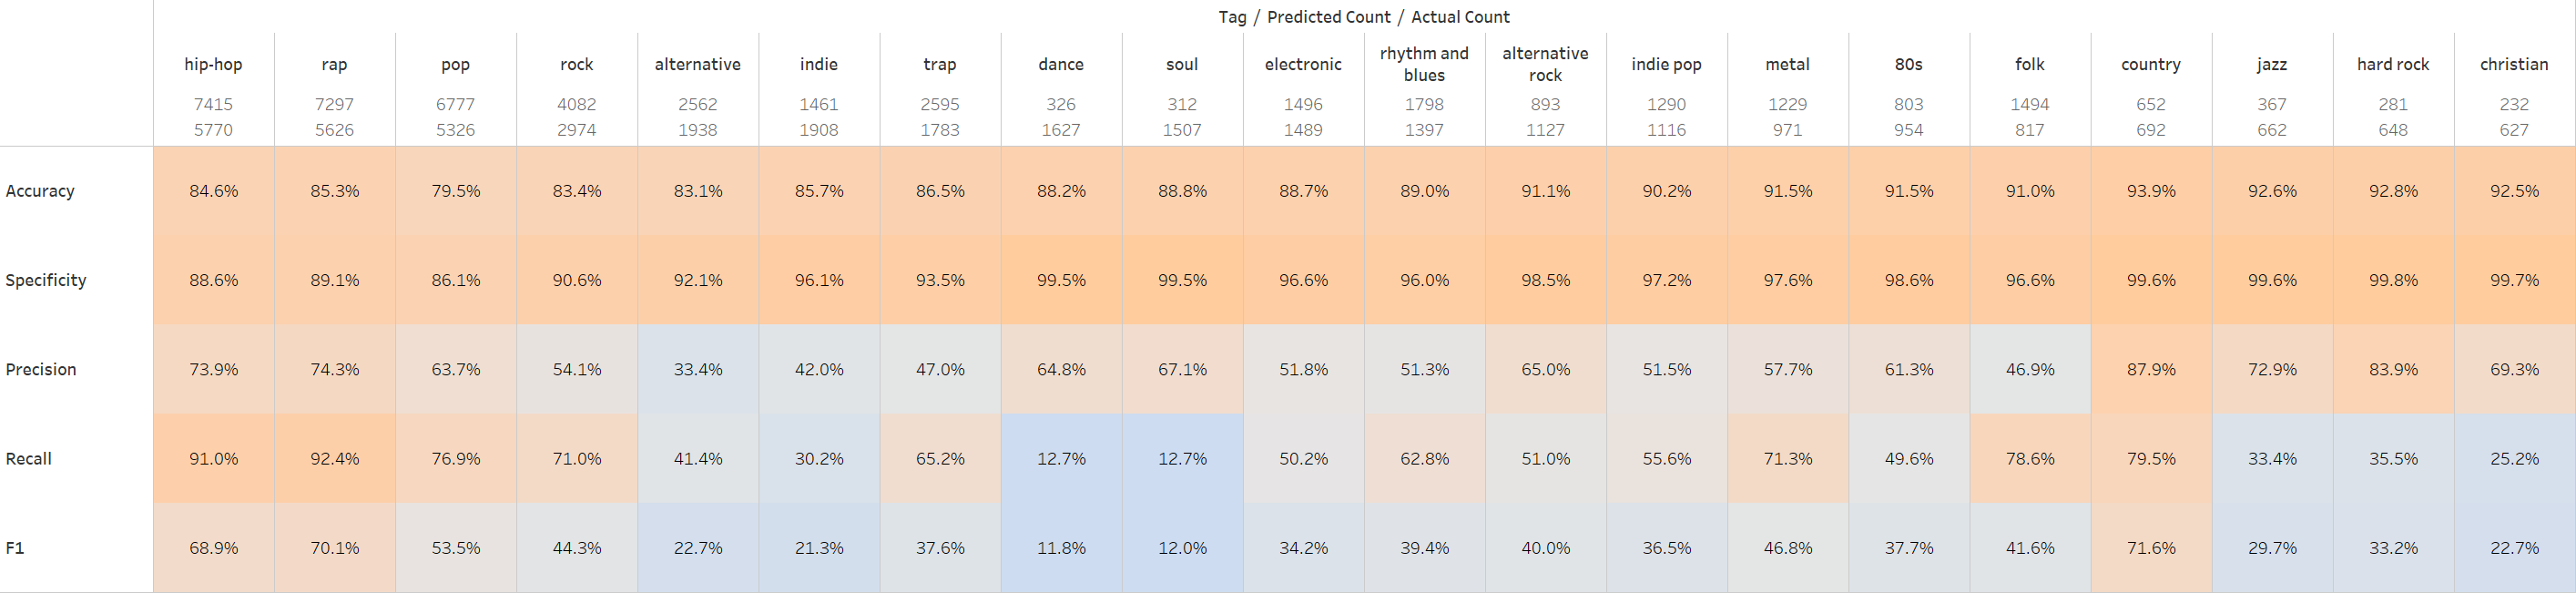
\includegraphics[width=\textwidth]{media/Scores.png}   
    \caption{Scores for top 20 tags by actual count ordered by actual count}
    \label{fig:finetune_scores_top20}
\end{figure}

\begin{multicols}{2}
\end{multicols}



\begin{figure}[h]
    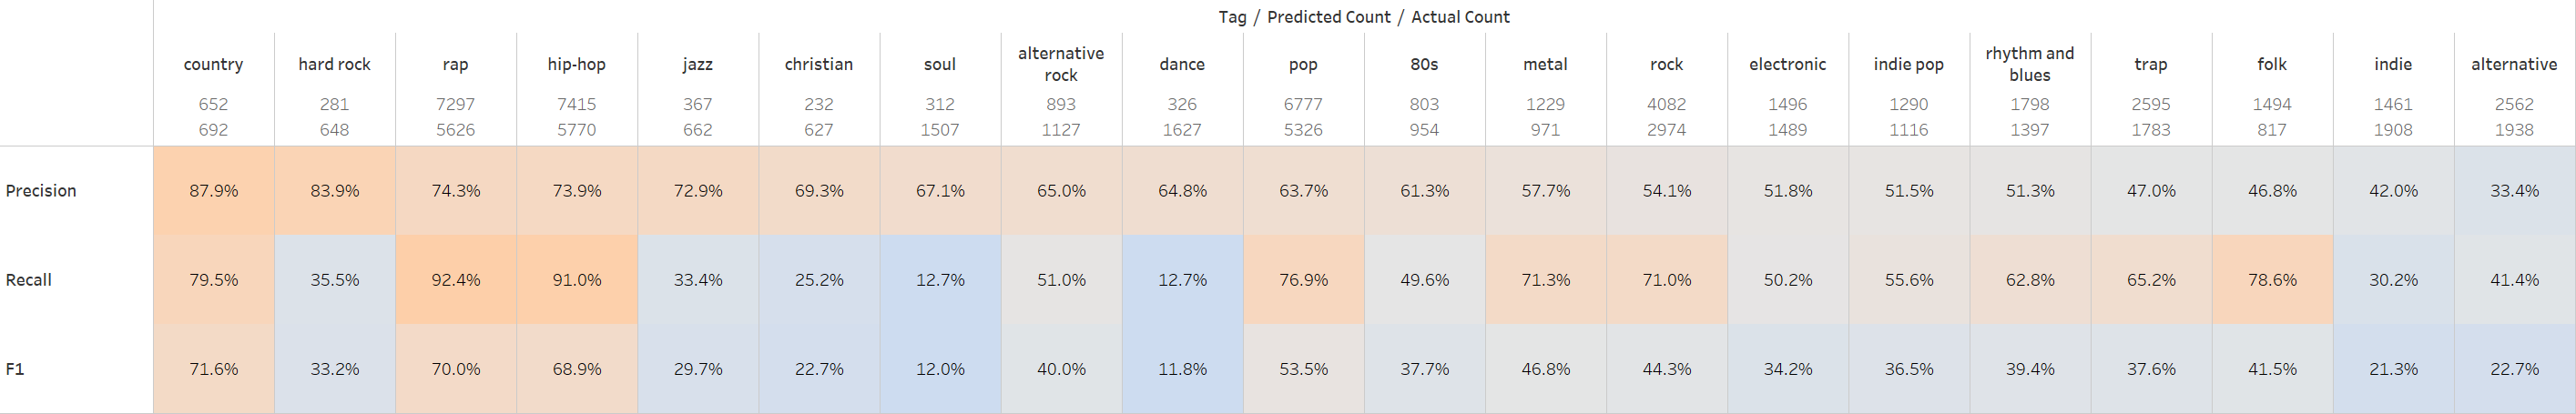
\includegraphics[width=\textwidth]{media/Scores By Precision.png}   
    \caption{Scores for top 20 tags by actual count ordered by precision}
    \label{fig:finetune_scores_top20_precision}
\end{figure}

\begin{figure}[h]
    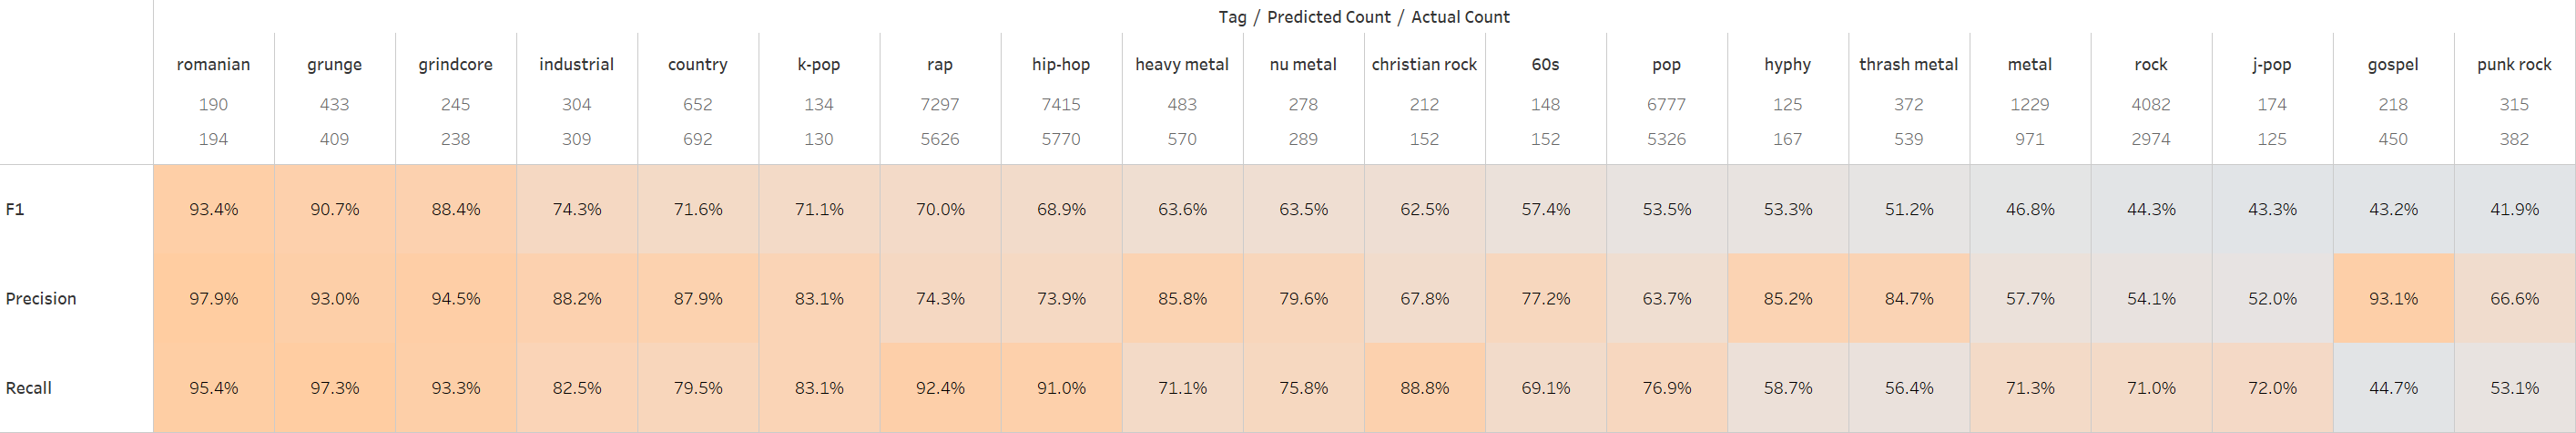
\includegraphics[width=\textwidth]{media/Scores By F1.png}   
    \caption{Scores for top 20 tags by F1 and > 100 actual count ordered by F1}
    \label{fig:finetune_scores_top20_f1}
\end{figure}

\begin{figure}[h]
    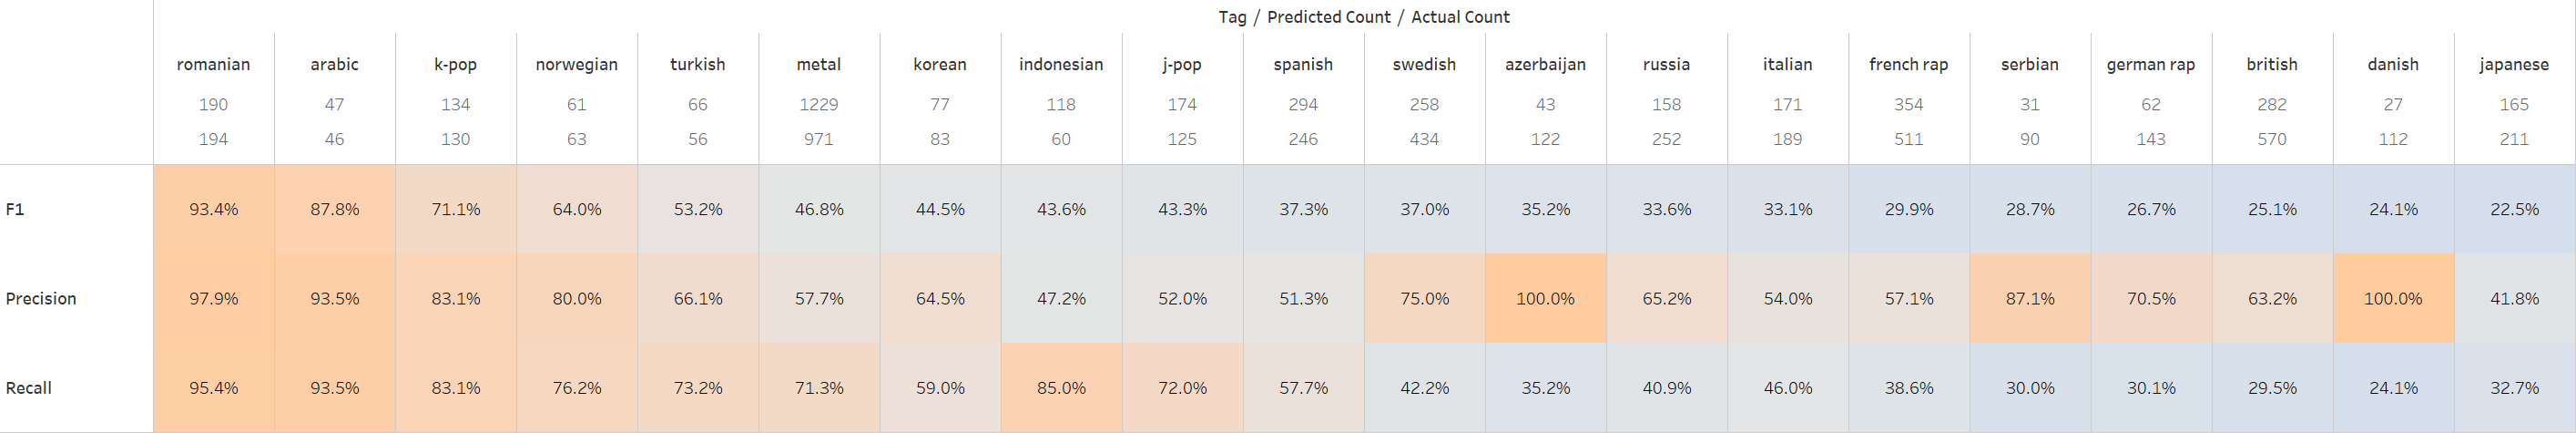
\includegraphics[width=\textwidth]{media/Scores For Languages.png}   
    \caption{Scores for top 20 language related tags by F1}
    \label{fig:finetune_scores_languages}
\end{figure}


\begin{multicols}{2}
Based on this, looking at the tags ordered by precision (\autoref{fig:finetune_scores_top20_precision}) suggests that the the genres: country, hard rock, rap, hip-hop, jazz, soul, alternative rock as well as christian themed music can be well identified by their lyrics. This assumption further can be confirmed by genres like dance or electronic which lay stronger emphasis on melody.

For the overall best tags (\autoref{fig:finetune_scores_top20_f1}) the model performs well at predicting languages (\autoref{fig:finetune_scores_languages}) of songs. Especially the more important\footnote[9]{In the tagging of songs, it is more important that the assinged tags are correct then finding all tags} precision score is overall $\sim70$\% for the top 20 tags by count and languages. Looking at the false negative songs\footnote[10]{out of scope for this paper, see the attached git repository \url{https://github.com/Aeolin/tag-me-up-daddy/tree/master/confusion/cm_record_including_songs.json} for further investigation} many stem from wrong or lacking last.fm tags where the model actually predicted the right tag but it was not included in the labels.

\subsection{Model Performance}



\begin{Figure}
    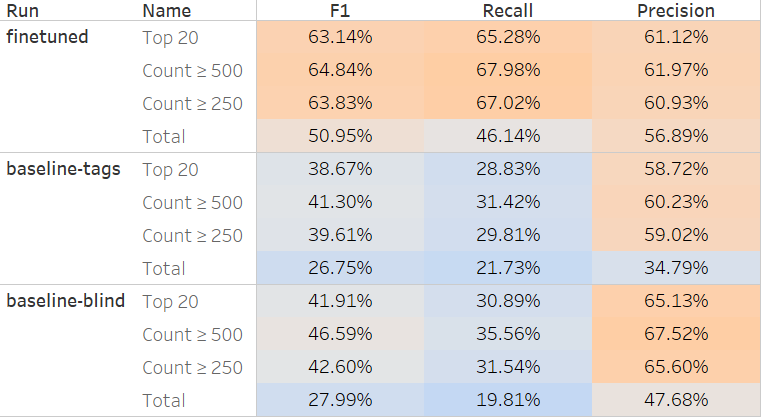
\includegraphics[width=\textwidth]{media/Run Comparison.png}
    \captionof{figure}{Comparison of approaches}
    \label{fig:comparison}
\end{Figure}

According to (\autoref{fig:comparison}) the fine tuned model performs best overall. The high precision scores are explicable by the exclusion of any non curated tags, even when counting false positives. Surprisingly the baseline which was given all available tags performed worse than the base line without any assistance. We highly suspect that the reason for this is an overfilled prompt, since for the baseline with tags gets a list of all curated 429 tags in it's system prompt.

\section{Discussion}

The single biggest mistake made during the evaluation and training was the oversight of unclean last.fm tags. It is highly suggested when recreating our approach to clean the tags before the fine tuning and evaluation as wells as removing all songs not containing a single tag after filtering from the dataset.

Another approach we want to test in the future is to crawl a more diverse dataset in terms of artist count, Or at least only use the lyrics, to prevent over fitting due to recognition of the artists name.

Overall the results, even tough the sub optimal dataset, look very promising and further investigation into song tagging with the use of fine tuned large language model is definitely viable.

\end{multicols}
\pagebreak
%-------------------------
% literature
%-------------------------
\bibliography{library}

\end{document}